\section{Propulsion} \label{section:propulsion}
\subsection{Introduction} % TODO: hyperlink reqs

The key responsibility of the propulsion system is to propel the rocket to the K\'{a}rm\'{a}n line utilizing two separate stages, each having their own individual motor (PRO.1 and PRO.2). Quantitative requirements that each motor will need to fulfill are being determined through Pareto analysis and the 6DOF model. The two point designs and the results of our analysis determine the specific aspects of the propulsion system. The team will thoroughly verify the ability of the propulsion system to complete the mission through simulation and testing. Each stage will contain its own ignition motor made of the same formulation as the main motor. While the first stage ignition will be manually activated by the mission control room, the second stage will be ignited by the avionics system on the second stage.

The formulation for each of the rocket motors and igniters is based on NATO propellant research~\cite{butacene} and will be carefully mixed and manufactured at Purdue University's propulsion laboratory --- Maurice J. Zucrow Laboratories. Through direct coordination with Zucrow, the propulsion team will construct a robust test stand in order to evaluate the performance of propulsion mechanisms and their interactions with other systems.

Throughout the research, design, manufacturing, and testing process, the team recognizes that it is paramount that safety is placed first, and is taking proper precautions to ensure this. We realize the inherent dangers of working with solid propellants and will work with experienced researchers to ensure the process is as safe as possible.


\subsection{Performance}
Two different point designs are currently being considered for the two-stage propulsion system based on system integration between the first and second stages. Currently, the primary difference between each design is the motor diameter. Variations and optimizations of the fuel grain geometry, the shape of the burning surface of the solid motor, will be determined after a point design is selected. Each point design was simulated based on each motor utilizing a BATES grain geometry (shown in \Cref{figure:segmented-grain}) with sub-minimum motor diameter. A CAD mockup is shown in \Cref{figure:bates-cad}. The quantitative requirements of performance for each design to achieve its mission were found through the thrust profiles from the 1DOF model and \(\Delta V\) outputs from the Pareto analysis. The first design considered has a first stage with an external diameter of 4.5 inches and a second stage with an external diameter of 4 inches. The second design consideration has a first stage with an external diameter of 5.5 inches and a second stage with an external diameter of 4.75 inches. The performance of each design is displayed in \Cref{table:prop-pareto-results}.

\begin{figure}
    \centering
    \includegraphics[width=0.6\textwidth]{images/segmented-propellant-grain}
    \caption{Section view of a segmented BATES grain (from \cite{zeller})} %
    \label{figure:segmented-grain}
\end{figure}

\begin{figure}
    \centering
    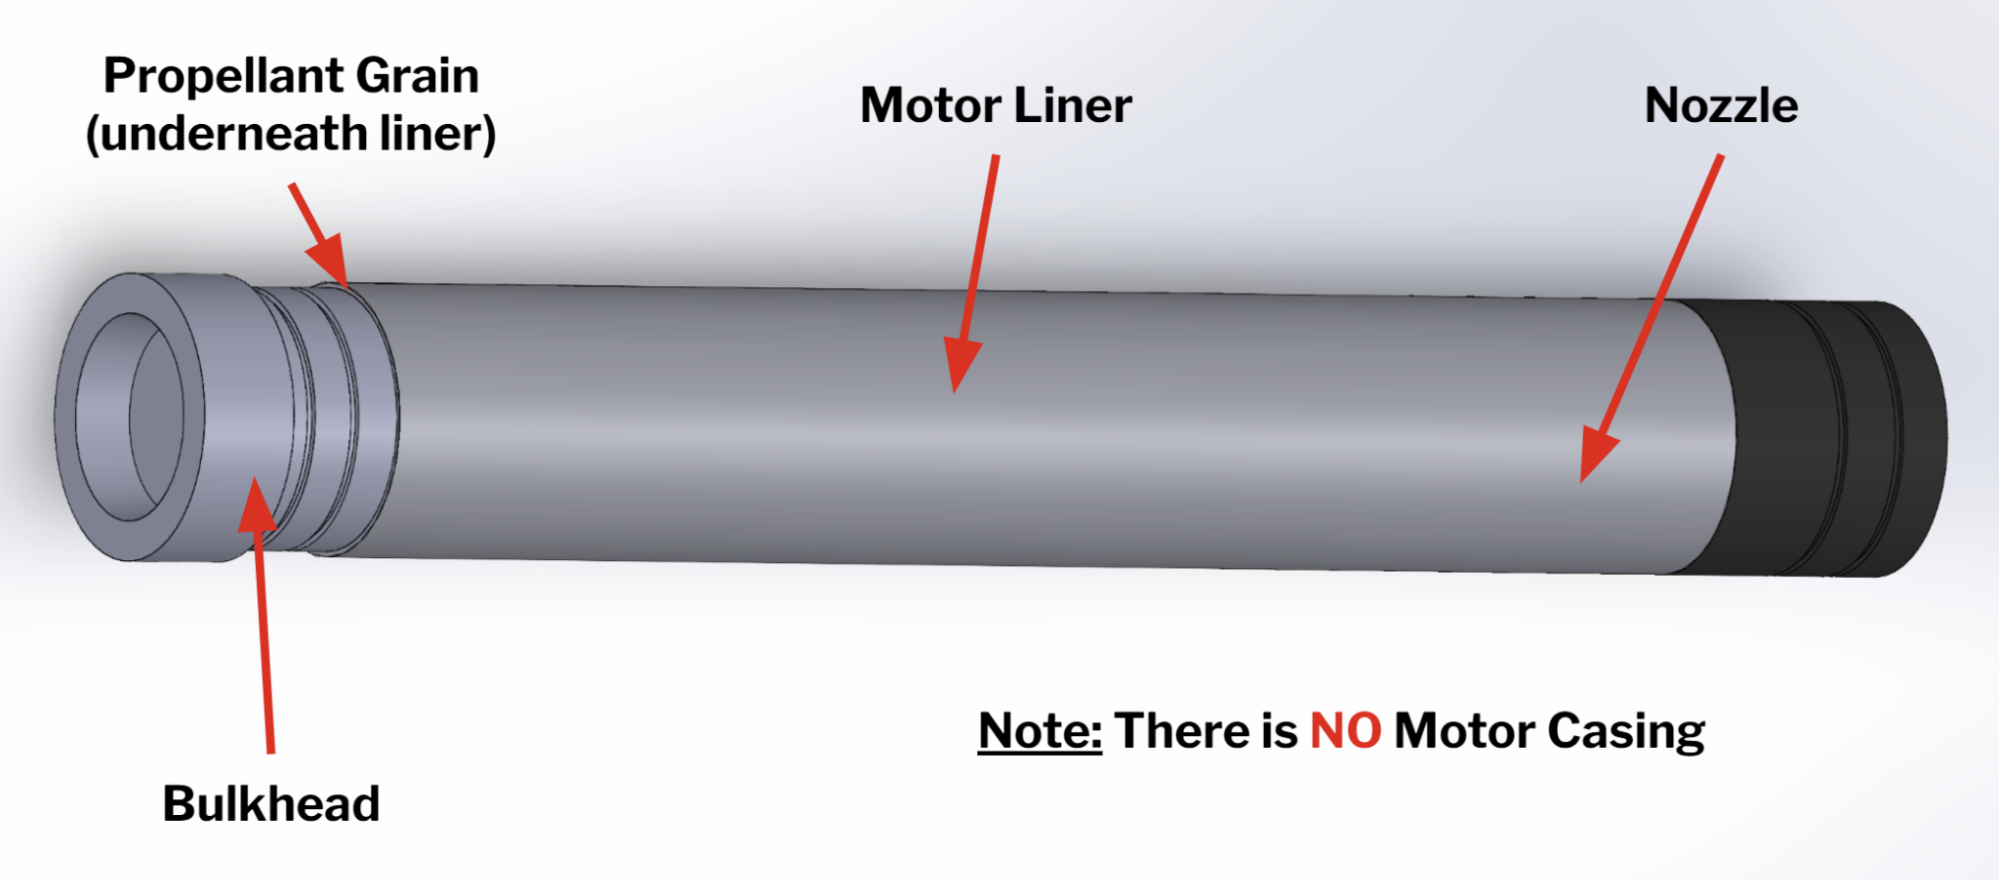
\includegraphics[width=0.75\textwidth]{images/prop-cad}
    \caption{CAD mockup of a sub-minimum diameter BATES motor assembly}
    \label{figure:bates-cad}
\end{figure}

\begin{table}
    \centering

    \begin{tabularx}{0.9\textwidth}{|p{2.5cm}|p{2cm}|p{3cm}|X|X|}
        \hline
        \multicolumn{5}{|c|}{\textbf{4'' - 4.5'' Design}} \\ \hline
        Burn Time (s) & \(\Delta V\) (km/s) & \(\Delta V\) Split (Stage 1) & \multicolumn{2}{|l|}{Impulse Requirement (N\(\cdot\)s)} \\ \hline
        \multirow{3}{*}{6 - 9} & \multirow{3}{*}{3.7 - 3.8} & \multirow{3}{*}{42.5\%} & Total & \(\sim\) 80\(\,\)000 \\ \cline{4-5}
        & & & Stage 1 & \(\sim\) 60\,000 \\ \cline{4-5}
        & & & Stage 2 & \(\sim\) 20\,000 \\ \hline        
    \end{tabularx}

    \vspace{0.75cm}

    \begin{tabularx}{0.9\textwidth}{|p{2.5cm}|p{2cm}|p{3cm}|X|X|}
        \hline
        \multicolumn{5}{|c|}{\textbf{4.75'' - 5.5'' Design}} \\ \hline
        Burn Time (s) & \(\Delta V\) (km/s) & \(\Delta V\) Split (Stage 1) & \multicolumn{2}{|l|}{Impulse Requirement (N\(\cdot\)s)} \\ \hline
        \multirow{3}{*}{7 - 9} & \multirow{3}{*}{3.4 - 3.5} & \multirow{3}{*}{35\%} & Total & \(\sim\) 100\(\,\)000 \\ \cline{4-5}
        & & & Stage 1 & \(\sim\) 56\,000 \\ \cline{4-5}
        & & & Stage 2 & \(\sim\) 44\,000 \\ \hline        
    \end{tabularx}

    \caption{Quantitative propulsion results of the Pareto analysis for both point designs}
    \label{table:prop-pareto-results}
\end{table}

\subsection{Ignition}
Ignition of both stages will be achieved through small ignition motors in their respective forward bulkheads (PRO.1.2, PRO.2.2). These ignition motors will be made of a faster-burning propellant than the main motors with a smaller-scale nozzle and casing to account for the change in atmospheric conditions at high altitudes. The igniters themselves will be ignited with a small pyrotechnic ignition charge.  Ignition of the first stage will be controlled via a wired connection to the control room. A manual key will be used for safety to inhibit unplanned ignition. The second stage will ignite via on-board avionics. This will be disarmed on the pad and remotely armed via an actuator with a physical key in the airframe. The actuator will be able to arm and disarm the second-stage ignition system remotely. 

When the second stage ignites, a burst disk will be applied on the nozzle to keep atmospheric pressure in the combustion chamber. While optimal separation is through drag separation, if an event occurs where this does not happen, stages will separate using the thrust from the second-stage motor. This will be discussed further in \Cref{section:interstage-mech}.


\subsection{Manufacturing}

\begin{table}
    \centering

    \begin{longtable}{|>{\raggedright\arraybackslash}p{5.75cm}|>{\raggedright\arraybackslash}p{8.75cm}|}
        \hline
        \multicolumn{1}{|c|}{\textbf{Hazard}} & \multicolumn{1}{c|}{\textbf{Mitigation}} \\ \hline
        Unwetted micrometric and nanometric metals pose an aerosol inhalation hazard & Any fine (micron) powders should be added inside of the ZL6 fume hood. Add metals and fine oxidizer close to the binder surface and wet thoroughly by hand stirring. \\ \hline
        Unwetted micro-metals pose an electrostatic discharge ignition hazard & Wear wrist ESD grounding straps during weighing and addition of micrometals. \\ \hline
        Ammonium perchlorate exposure can cause kidney and thyroid damage & Use a ceiling mounted high-volume draft fan operating at 100\% flowrate during the entire mixing procedure. \\ \hline
        Isocyanates used as curatives are highly neurotoxic and are an inhalation hazard & Use low vapor pressure isocyanate. Any isocyanate will be weighed out and added to the mixing bowl within the ZL6 fume hood. \\ \hline
        Skin absorption of propellants can be toxic to operator & Wear appropriate nitrile gloves and safety glasses for the entire procedure. In case of contact, flush out the area of the skin with water and follow propellant material safety data sheets for further instructions. \\ \hline
        Ignition of propellant in bowl during mixing & Mixing will be conducted away from any flammable materials. No smoking or open flames will be permitted in the mixing cell. \\ \hline
        Waste presents fire and toxicity hazard & Dispose of any excess propellant or contaminated material through Purdue's REM. \\ \hline
    \end{longtable}

    \vspace{0.2cm}
    
    \caption{Hazards present in the mixing process, and mitigation plans}
    \label{table:prop-hazards}
\end{table}

Motors will be mixed at Zucrow Labs, in building ZL6 using the Hobart 20 qt dough mixer. All fine powders will be measured in a fume hood with wrist ESD grounding straps to prevent ignition. Pants, lab coats, nitrile gloves, and eye protection will be worn during every stage of the mixing process. Solids will be carefully wetted in increments. Propellant will be vacuum processed after mixing/before casting to evacuate air bubbles. Propellant will be pourable and cast into Kraft paper tubes around a removable mandrel to form the grain shape. Paper tubes are used for inhibition of the outer surface. Grains will be cast longer than needed and cut to the exact length for propellant consistency. Grains will be glued into the phenolic motor insulator, and the grain faces will be cut concavely to prevent accidental face inhibition.

All mixing operations will be performed under the supervision of Tim Manship or an approved Zucrow graduate student. All waste propellants and chemicals will be disposed of in accordance with the Purdue Radiological and Environmental Management (REM) requirements \cite{rem-disposal}. Hazards and mitigation relevant to the mixing procedure are discussed in the \Cref{table:prop-hazards}.


\subsection{Testing}
The objectives of the testing process will be to confirm the safe operation of the propulsion system and to verify its ability to meet our performance requirements. The first phase of testing will be propellant formula characterization. The second phase will include the creation of a test stand in direct collaboration with Zucrow Laboratories and motor testing of our propellant. The test stand design will incorporate elements found in industry and academic test stands to maximize safety and simplicity. The team will utilize an iterative testing process where small-scale tests are conducted to confirm prior analysis and modeling before building upon the data to create larger-scale and more comprehensive tests.

Propellant formula will be characterized through pressure bomb strand-burning analysis to obtain the burn rate coefficient and exponent. This testing will be completed under existing safety procedures at Zucrow Laboratories and manufacturing of strands will be completed safely as outlined in our manufacturing section. Example safety procedures are provided in \Cref{section:prop-appendix}. Along with strand burning, tensile testing of propellant dog bones will help confirm the propellant formulation exhibits the required mechanical properties to complete the mission, such as the propellant's tensile strength.

After small-scale propellant testing, a subscale single-grain Bates motor cast with our propellant will be tested to confirm predicted chamber pressures and thrust based on modeling and simulation. Finally, full-scale motors will be tested before launch to confirm that systems work nominally on a large scale and are capable of achieving the required total delta V (PRO.1.1.4, PRO.2.1.4) and thrust profile. Effects of the propulsion system on other subsystems will be tested to confirm that heat generated by the motors does not deteriorate the integrity of the rocket structure. Additional tests will indicate how quickly and effectively the second-stage igniter can accept the fire signal from the avionics system.

A horizontal test stand will be used to experimentally verify the thrust (delay, duration, and maximum) and chamber pressure values predicted by the simulations subteam. The majority of solid motors in industry are tested horizontally as this is typically safer in the event of a test stand failure. Mounting motors horizontally eliminates the need for any actions to be performed on an elevated surface because the entire motor is close to the ground. This simplifies testing setup and limits the time spent in close proximity to energetics. Solid motor performances are also not significantly affected by gravity, so it is not necessary for the team to create a vertical test stand which simulates the proper launch orientation.

\begin{figure}
    \centering
    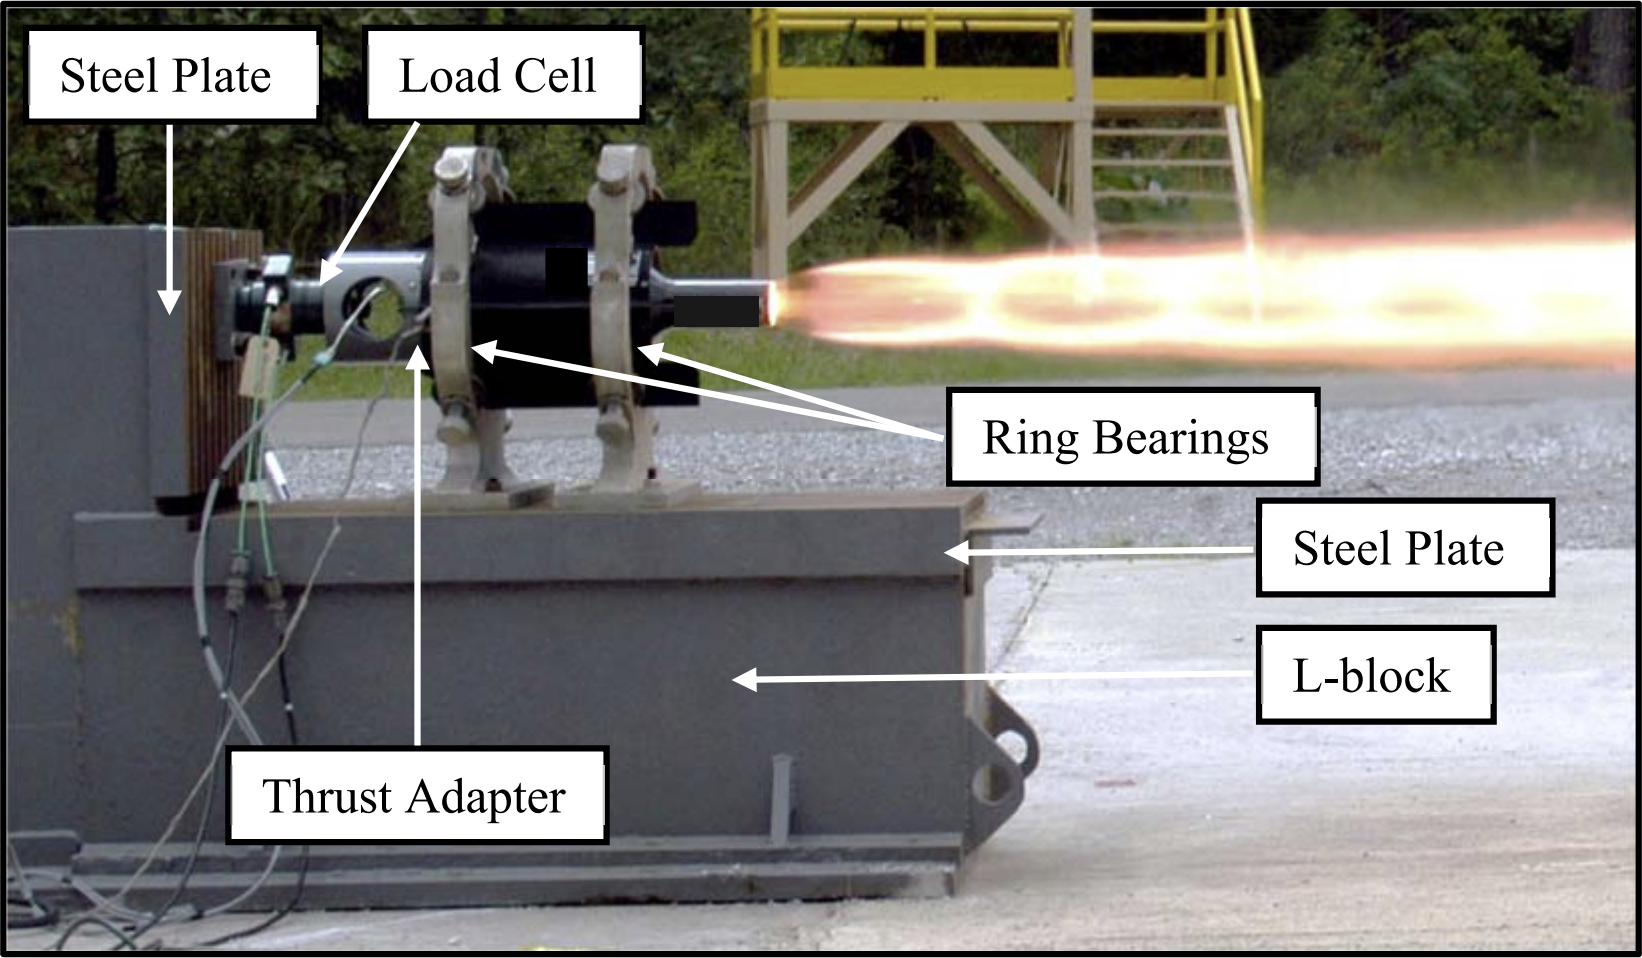
\includegraphics[width=0.6\textwidth]{images/srm-mobile-lblock}
    \caption{Solid rocket motor firing from a mobile L-lock (from \cite{uah-thesis})}
    \label{figure:lblock1}
\end{figure}

\begin{figure}
    \centering
    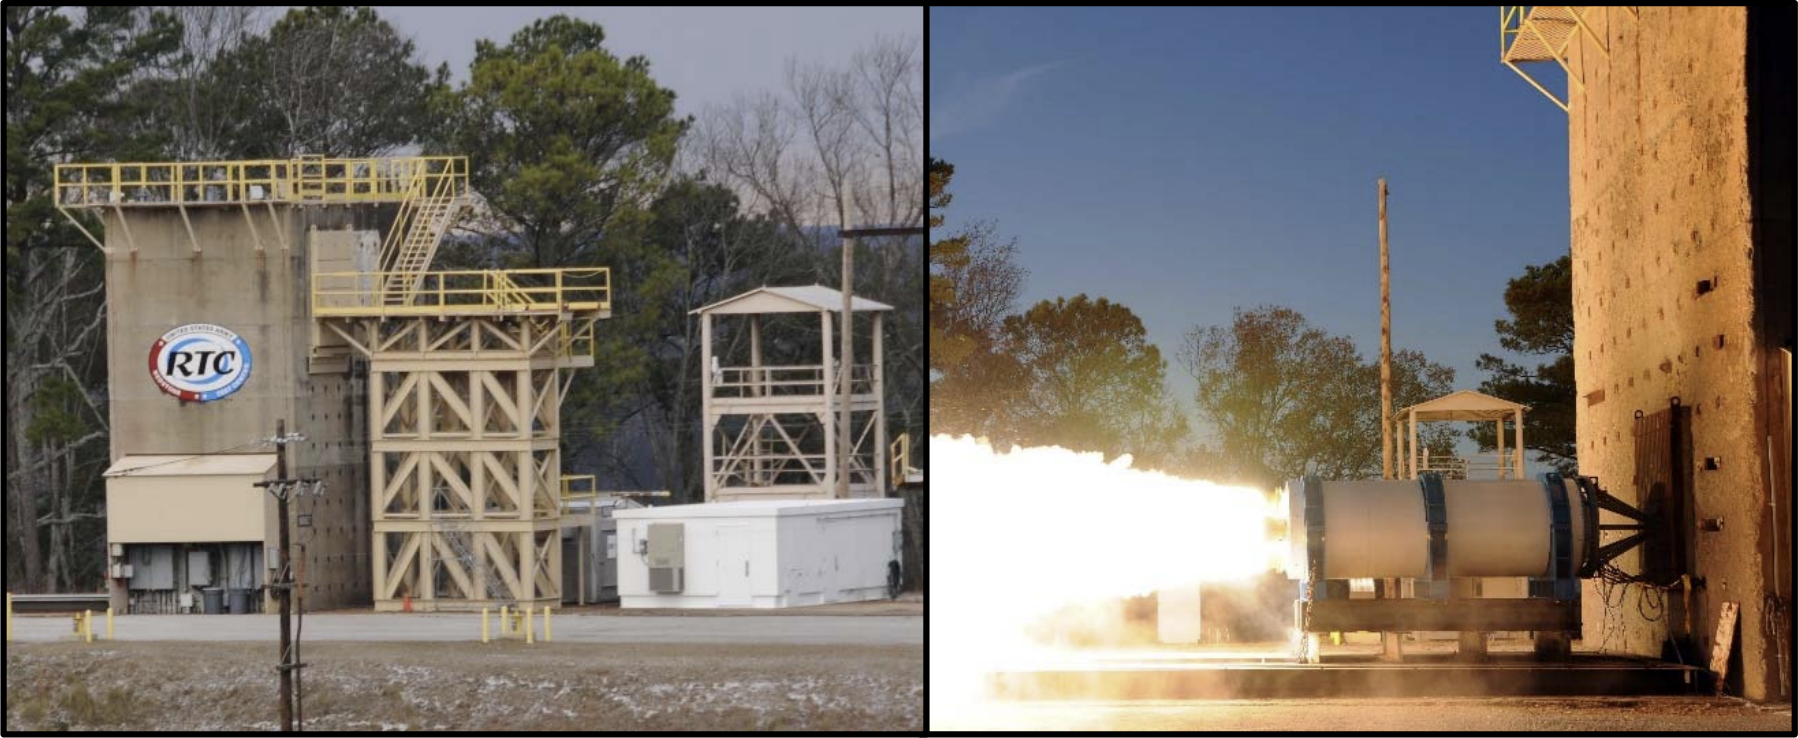
\includegraphics[width=0.6\textwidth]{images/srm-firing}
    \caption{Solid rocket motor firing from a fixed L-lock (from \cite{uah-thesis})}
    \label{figure:lblock2}
\end{figure}

To verify the safety of our testing systems, research has been conducted into prior test stand designs that are centered around an I-beam assembly. One of the more well-documented I-beam test stand designs is that of the University of Alabama Huntsville. The university has created two similar L-block designs, with the key difference between them being that one features a mobile L-block (\Cref{figure:lblock1}) while the other features a fixed L-block (\Cref{figure:lblock1}). The mobile L-block is employed when testing small, tactical-size motors and can be placed at several different locations within their facility campus depending on the test objectives. By contrast, the fixed L-block is a monolithic reinforced concrete/rebar block that is embedded up to 50 feet below grade and surrounded by a concrete apron, which acts as the horizontal ``L'' face. The main component of the horizontal face is a rail system based around an I-beam that can accommodate motor-firing carts of different sizes.  The vertical ``L'' face is reinforced with concrete and a large, 6-inch-thick steel plate to support the motor and handle high thrust forces during firing \cite{uah-thesis}.

\begin{figure}
    \centering
    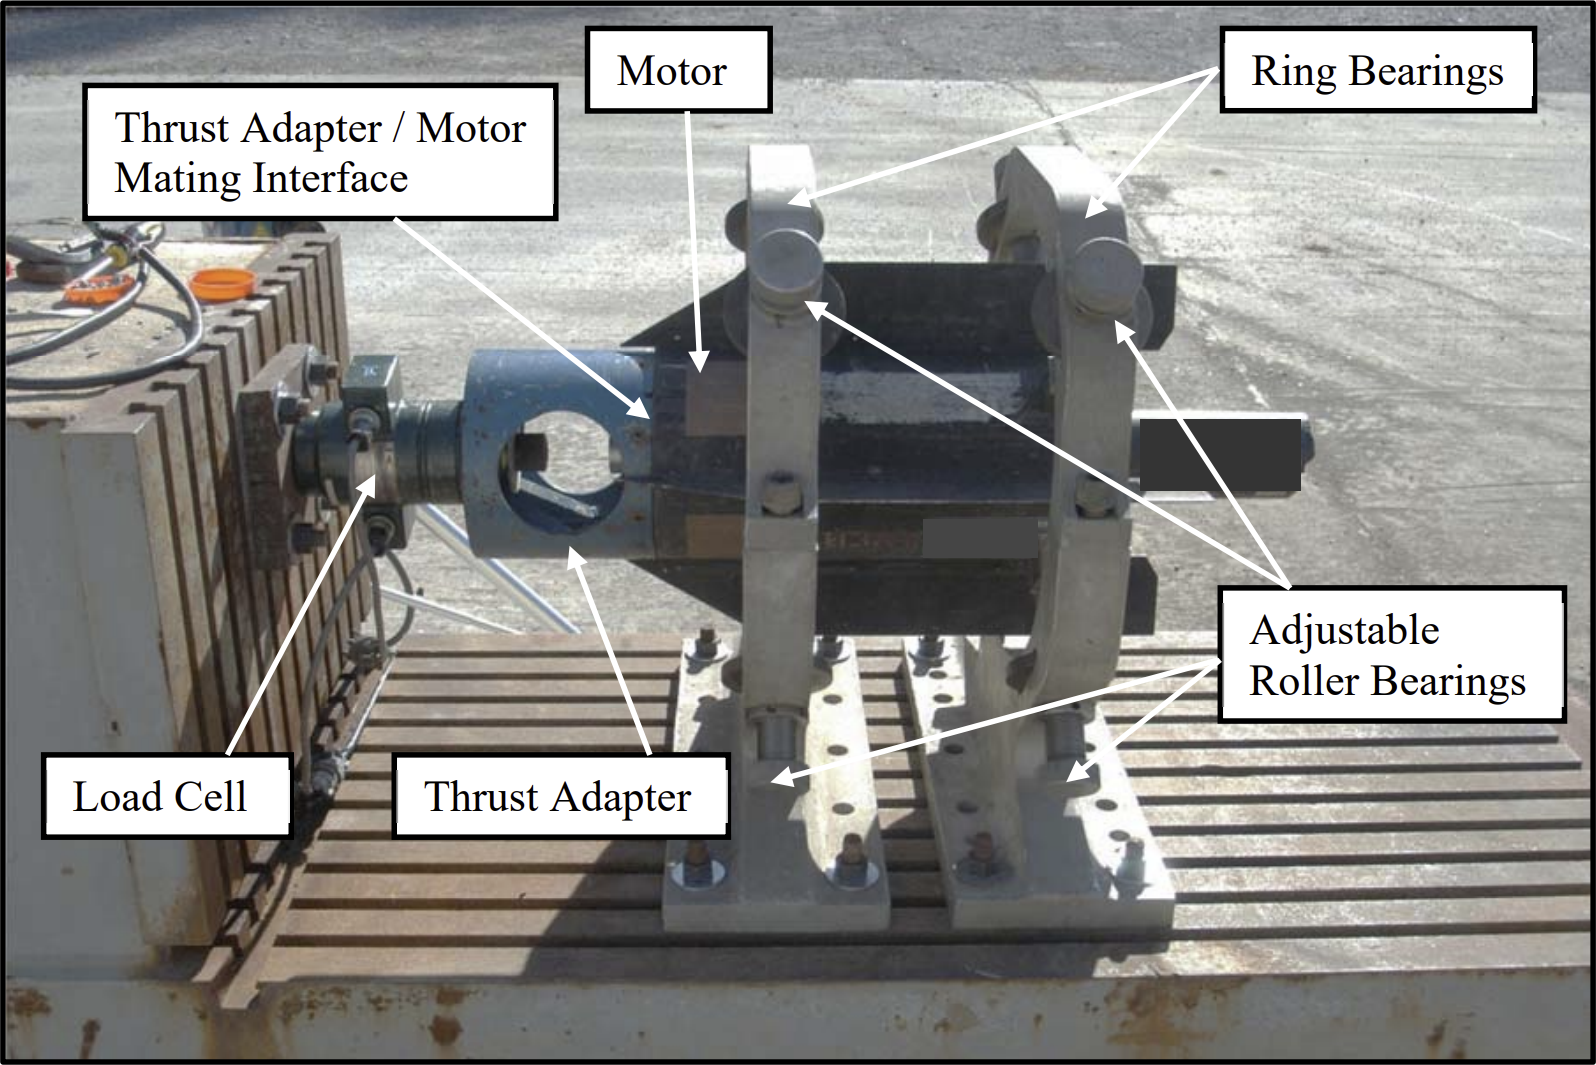
\includegraphics[width=0.6\textwidth]{images/ring-roller-bearing}
    \caption{Ring / roller bearing arrangement used for leveling and centering (from \cite{uah-thesis})}
    \label{figure:rollerbearing}
\end{figure}

\begin{figure}
    \centering
    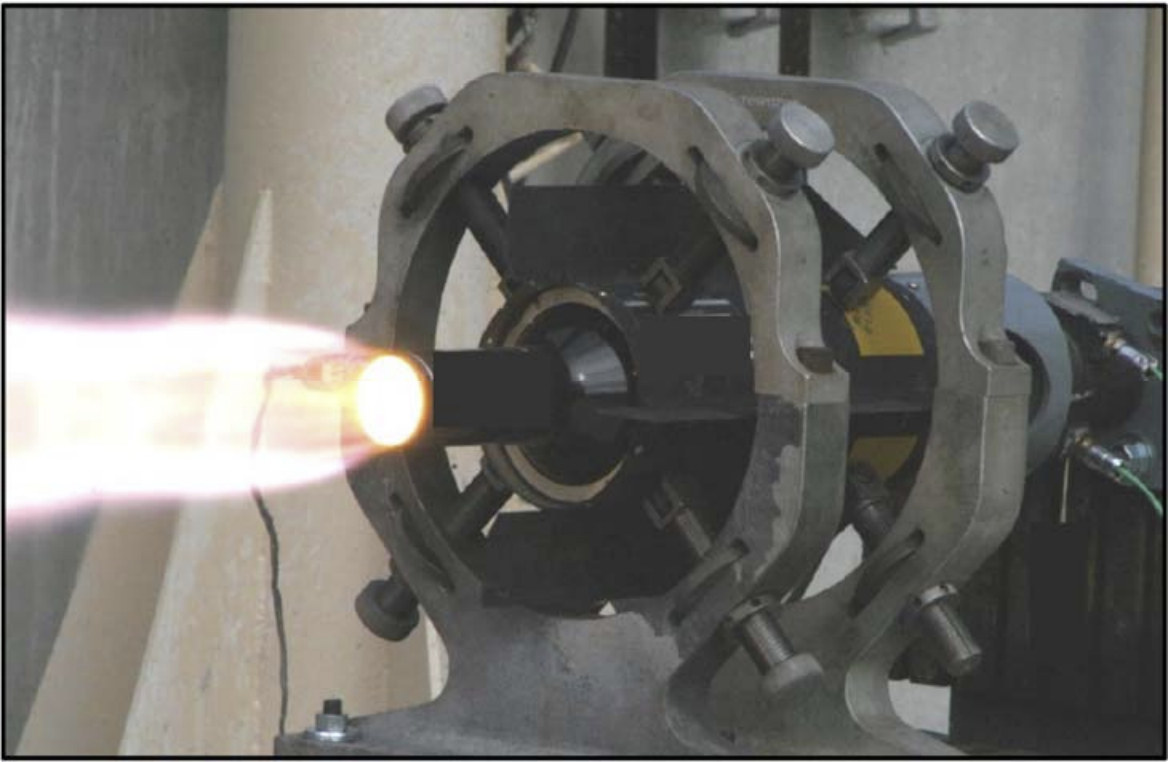
\includegraphics[width=0.6\textwidth]{images/static-motor-firing}
    \caption{Typical static motor firing (from \cite{uah-thesis})}
    \label{figure:firing}
\end{figure}

Prior to motor installation, the L-block is prepared with measurement tools suited for the motor being fired. The appropriate load cell, thrust adapter, ring bearings, and various other specific attachment hardware are installed (\Cref{figure:rollerbearing} and \Cref{figure:firing}). Next, a mock motor of the proper dimensions is installed to ensure preliminary centering and leveling with the centerline of the load cell and thrust adapter. Installing a motor in the system involves using adjustable cylindrical roller bearings which contact the motor case and allow free axial motion of the motor. Following this initial process, a live motor is installed in place of the mock motor, with the centering and leveling fine-tuned (involving close monitoring of the distribution of light around the motor in the interface between the thrust adapter and the motor) before the motor is seated into the thrust adapter and bolted in place. After arming the motor, all testing operations personnel must return to the control room to begin the static fire. Safety is further ensured through FEA determination of the maximum yield stress beforehand. Strain gauge-based canister load cells measure the motor thrust by means of electrical signals, with a larger signal correlating with a larger thrust force \cite{uah-thesis}.

\begin{table}
    \centering

    \begin{longtable}{|>{\raggedright\arraybackslash}p{5.75cm}|>{\raggedright\arraybackslash}p{8.75cm}|}
        \hline
        \multicolumn{1}{|c|}{\textbf{Hazard}} & \multicolumn{1}{c|}{\textbf{Mitigation}} \\ \hline
        Snap ring assembly & Wear safety glasses and work gloves when installing snap rings. Cup tensioned snap ring with hands while installing and point snap ring away from people. \\ \hline
        Mounting brackets are heavy and may pose a hazard when suspended & Require a minimum of two people to lift any heavy objects. \\ \hline
        Early, unintended ignition of test motor & Keep ignition circuit isolated until the motor is ready for testing. Keep any flames or heat sources away from propellant grains. \\ \hline
        Catastrophic motor failure & Ensure all testing is conducted remotely, with appropriate stand-off distances or bunkers in place. Fire suppression systems must be easily accessible. \\ \hline
    \end{longtable}

    \vspace{0.2cm}
    
    \caption{Hazards present during hot fire testing, and mitigation plans}
    \label{table:hotfire-hazards}
\end{table}

In addition to rigorous verification of the design of our test systems, we must verify the safety of our procedures. We will refer to existing Zucrow Laboratories procedures to create new procedures for motor assembly and hot-fire. Alongside instructions needed to conduct the test, the procedures will include appropriate PPE to be used; potential hazards and mitigation, such as limiting smoking and open fires near flammable objects; and lastly any additional procedures needed in case of a safety incident such as an occurrence of fire on the test setup. Any fire will not be fought. Instead, the building will be evacuated and emergency contacts will be approached. Hazards specific to each test will have additional safety requirements, given in \Cref{table:hotfire-hazards}, \Cref{table:dogbone-hazards}, and \Cref{table:bomb-hazards}.

\begin{table}
    \centering

    \begin{longtable}{|>{\raggedright\arraybackslash}p{5.75cm}|>{\raggedright\arraybackslash}p{8.75cm}|}
        \hline
        \multicolumn{1}{|c|}{\textbf{Hazard}} & \multicolumn{1}{c|}{\textbf{Mitigation}} \\ \hline
        Toxic chemicals, aerosol sprays & Use aerosol sprays in well-ventilated spaces and avoid breathing in aerosolized mist. \\ \hline
    \end{longtable}

    \vspace{0.2cm}
    
    \caption{Hazards present during dog bone testing, and mitigation plans}
    \label{table:dogbone-hazards}
\end{table}

\begin{table}
    \centering

    \begin{longtable}{|>{\raggedright\arraybackslash}p{5.75cm}|>{\raggedright\arraybackslash}p{8.75cm}|}
        \hline
        \multicolumn{1}{|c|}{\textbf{Hazard}} & \multicolumn{1}{c|}{\textbf{Mitigation}} \\ \hline
        Failure of pressurized parts & Test will be operated remotely from a control room. \\ \hline
        Ignition of energetics during handling and preparation & Use small sample sizes (<5g) and wear PPE. \\ \hline
        Post-experiment residue exposure & Purge pressure vessel with an inert gas after experiment. \\ \hline
    \end{longtable}

    \vspace{0.2cm}
    
    \caption{Hazards present during pressure vessel and Crawford bomb testing, and mitigation plans}
    \label{table:bomb-hazards}
\end{table}

Currently, any procedures created are provisional as designs are not finalized. All procedures will be revised accordingly to any design changes. Before any testing is conducted, safety procedures will be verified by Tim Manship and Scott Meyer. Additionally, subject matter experts Dr. Stephen D. Heister and Prof. Mark Grubelich will actively provide any feedback as they deem necessary. All members who will conduct tests shall fulfill Zucrow Laboratories training requirements that will be provided by Tim and Scott in addition to reviewing each test procedure.


\subsection{Analysis and Simulation}

As safety is of paramount concern, structural Finite Element Analysis (FEA) will be used during the design of the test stand and motor to ensure designs meet all safety requirements. FEA results combined with hand calculations will be used to determine bolt preloads, torques, and show that all components can handle expected loads scaled by safety factors while retaining a positive safety margin. The FEA models will be created and run using Siemens NX Nastran.

Once vehicle sizing has been completed, motor grains will be designed to match the optimal thrust vs time profile for the flight. Two Blackburn simulation programs are planned to be used for grain design. The initial design will be completed using BurnSim, a commercially available burnback program. Once an adequate base grain design has been determined, an in-house optimization program will be used to refine the geometry to its final state. The program is based on work done by Magni Johannsson \cite{magni} but will use different simulation programs. The optimizer will combine an NX (CAD-based) surface regression program with a MATLAB-based ballistic modeling script for thrust and pressure calculations, and a derivative-free local optimization program called NOMADS. 

The dual program approach will be used due to the runtime of each program and the lack of documentation on the calculation methods used by BurnSim. The quick run speed of BurnSim allows for rapid iterations of geometry with reasonable results before transitioning to our own ballistic code. Our code takes longer to run, but provides thrust and pressure results with more confidence as we know how calculations are being done.


\subsection{Combustion Modeling}
In order to properly model the internal combustion of a motor, relations were derived based upon quasi-one-dimensional flow relations and by utilizing a mass and momentum balance. This particular method tracks discrete elements in the combustion chamber as a function of time. By selecting the system to be the port of the motor, conservation of mass can be used as mass input from the propellant grain, and mass output through the nozzle of the rocket. This understanding along with isentropic relations builds the foundation of this model and is able to track the combustion processes to occur.

The core of this model revolves around discretized segments of the grain into a large number of elements, of which a sample element is shown below. In the schematic, each element adds a certain amount of mass to the exhaust gas in the port of the element, which then changes the total pressure, static pressure, and Mach number which leads to compressibility effects in the fluid. The amount of mass that is being added to the flow is dictated by the surface area of the propellant, which can be modeled as a function of web, while the Mach number is affected by the port's cross sectional area.

The key advantage of splitting each segment into elements is the ability to track the exhaust gas property changes as a function of axial distance down the motor, and by time. When run until termination of the program, this ability to track per element allows for the compilation of data as a time history for a simulated burn of the motor. This allowed for our team to match certain qualities of a motor to things such as grain geometry and chamber pressure, chamber pressure and thrust as a function of time, and other key propulsive performance metrics.

\begin{figure}
    \centering
    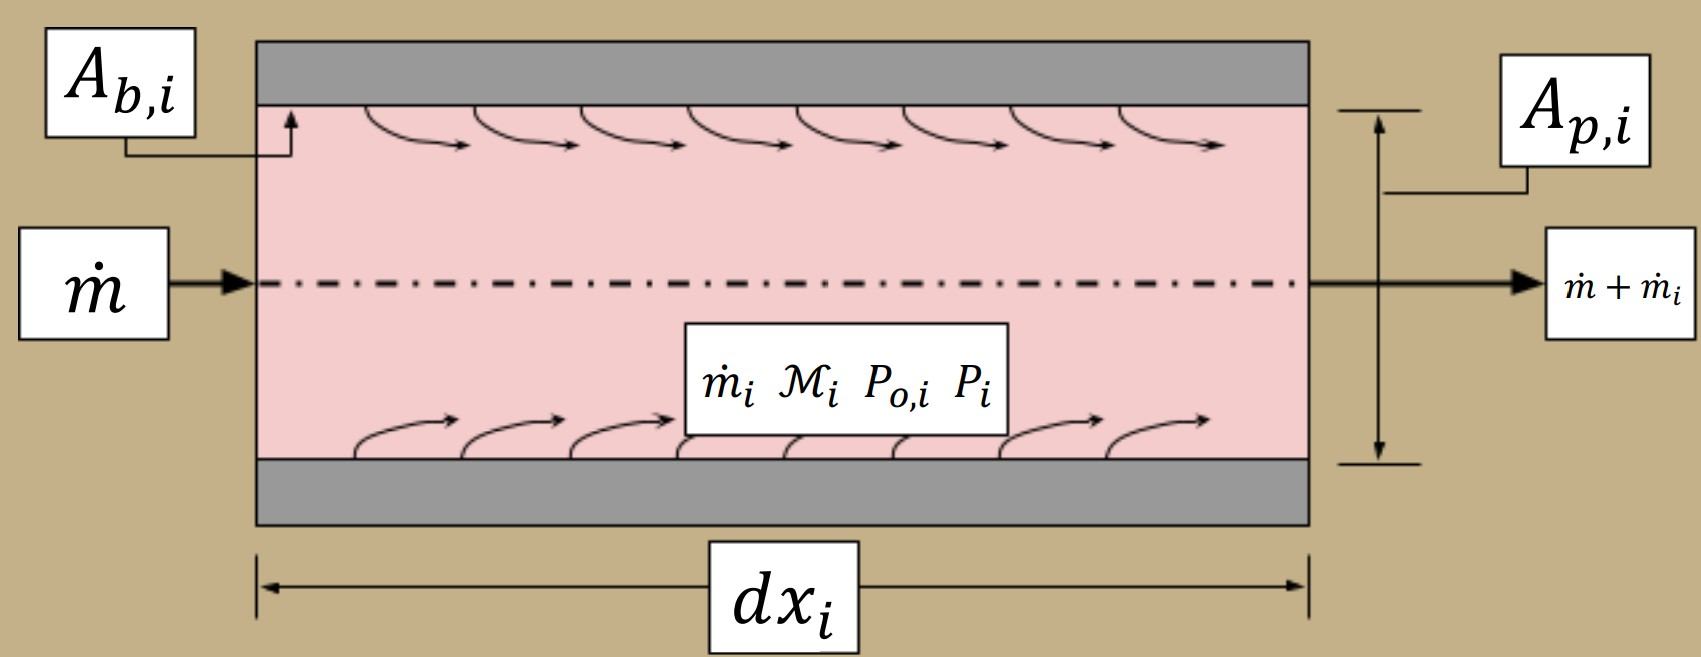
\includegraphics[width=0.8\textwidth]{images/combustion-diagram}
    \caption{Diagram of the control volume for solid rocket motor combustion analysis}
    \label{figure:combustion-diagram}
\end{figure}

The initial head pressure conditions are estimated with the Steady State Lumped Parameter model, shown in \Cref{equation:1}, which is then used to iteratively find a quasi-transient head chamber pressure. The program then steps axially through the elements of each segment and updates the flow properties as it goes, using Equations 2 through 5. Once the last element has been run, a mass balance is performed to check the amount of mass accumulated in the port to the theoretical mass that should have accumulated as dictated by \Cref{equation:8}. If the two values of mass were within a tolerance of one another, then a time step equal to half of the chamber time constant was taken which updated the geometry of the grain with the appropriate web based on the local stagnation pressure at each element. Additionally, NASA CEA was utilized to find local exhaust properties of each element based on the chamber pressure. When an element ``burned out'' meaning there was no more exposed propellant that had a surface area, then that element was treated as a slot. Each slot was modeled as a single element that had a stagnation pressure loss as found in \cite{heister-paper}. The program would terminate when all of the elements have burned to their maximum web or the stagnation pressure at the head of the motor was less than 200 psi (chosen to show the ending of the burn). The model algorithm structure can be found in \Cref{figure:combustion-flowchart}.

\begin{figure}
    \centering
    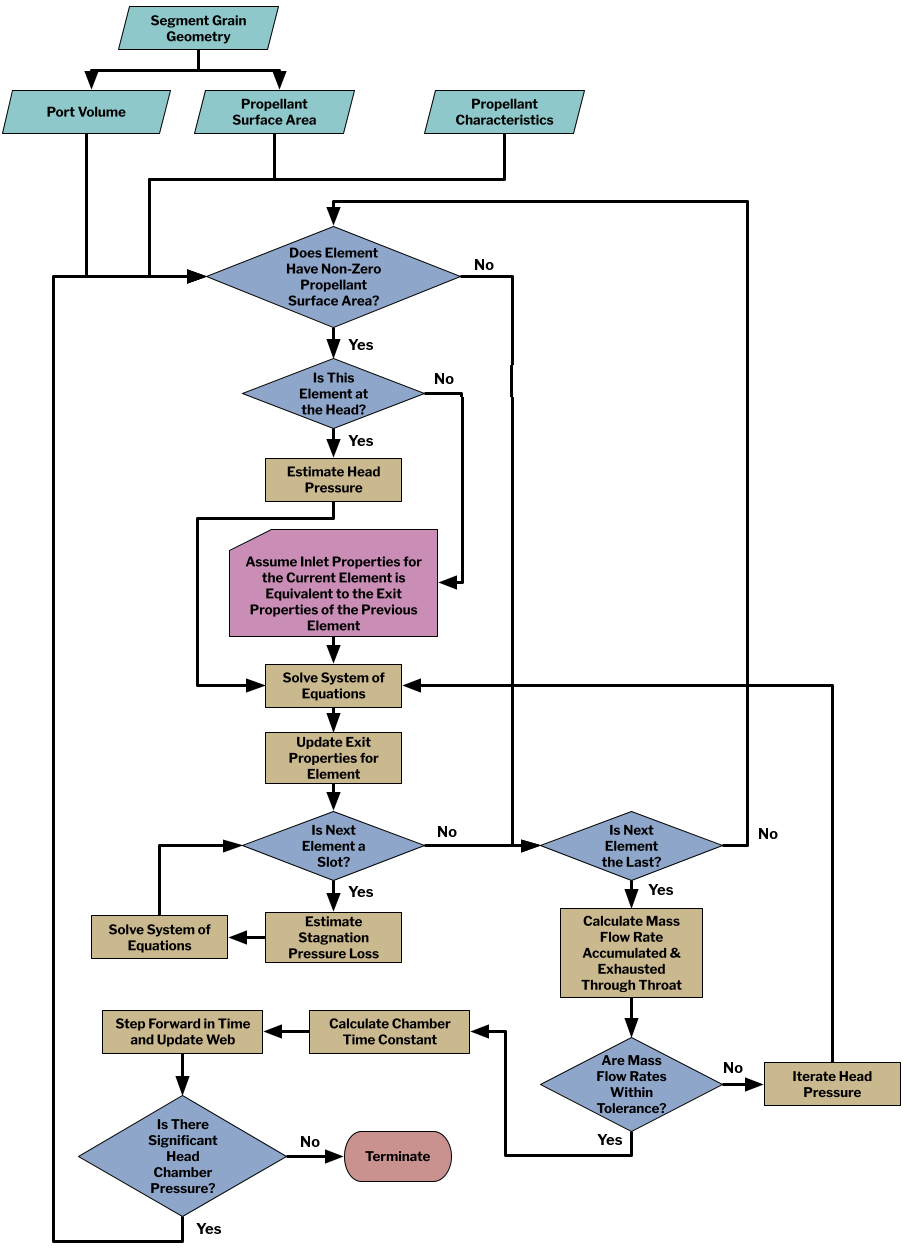
\includegraphics[height=0.9\textheight]{images/combustion-flowchart}
    \caption{Flow chart representing the ballistic model algorithm}
    \label{figure:combustion-flowchart}
\end{figure}

The algorithm solved the following equations as a system of equations for each element, via the following process.

\begin{enumerate}
    \item Solve \Cref{equation:2} for the mass input of that segment using the assumption that static and Mach number are the same as for the previous element
    \item Solve \Cref{equation:3} for stagnation pressure using the previous element's Mach number
    \item Solve \Cref{equation:4} for static pressure using the previous element's Mach number
    \item Solve \Cref{equation:5} for Mach number implicitly
    \item Resolve \Cref{equation:4} with updated Mach number for static pressure
    \item Resolve \Cref{equation:3} with updated Mach number and static pressure for stagnation pressure
    \item Resolve \Cref{equation:2} with updated stagnation pressure
\end{enumerate}

\begin{figure*}[htbp]
    \begin{equation} \label{equation:1}
        P_0 = \left(\frac{a \rho A_b c^*}{g A_t}\right)^\frac{1}{1-n}
    \end{equation}
    \caption*{Steady lumped parameter model (estimate head pressure)}
\end{figure*}

\begin{figure*}[htbp]
    \begin{equation} \label{equation:2}
        \dot{m}_i = a P_{o,i}^n \rho A_{b,i}
    \end{equation}
    \caption*{Continuity equation}
\end{figure*}

\begin{figure*}[htbp]
    \begin{equation} \label{equation:3}
        P_{0,i} = \frac{P_{i-1}}{1 + \gamma \mathcal{M}_i^2 \left(\frac{\dot{m}_i}{\dot{m}}\right)}
    \end{equation}
    \caption*{Momentum Equation}
\end{figure*}

\begin{figure*}[htbp]
    \begin{equation} \label{equation:4}
        P_i = \frac{P_{0,i}}{\left(1 + \frac{\gamma - 1}{2} \mathcal{M}_i^2\right)^\frac{\gamma}{\gamma - 1}}
    \end{equation}
    \caption*{Isentropic pressure relation}
\end{figure*}

\begin{figure*}[htbp]
    \begin{equation} \label{equation:5}
        \dot{m}_i + \frac{\dot{m}_i}{2} = \left(\frac{\mathcal{M}_i P_{0,i} A_{p,i}}{\sqrt{\frac{R T_c}{\gamma}}}\right) \left(1 + \frac{\gamma - 1}{2} \mathcal{M}_i^2\right)^\frac{-\gamma-1}{2(\gamma - 1)}
    \end{equation}
    \caption*{Average mass flow; is solved for Mach number (\(\mathcal{M}_i\))}
\end{figure*}

\begin{figure*}[htbp]
    \begin{equation} \label{equation:6}
        \dot{m}_{in} \sum_{i=1}^n \dot{m}_i
    \end{equation}
    \caption*{Mass accumulation}
\end{figure*}

\begin{figure*}[htbp]
    \begin{equation} \label{equation:7}
        \dot{m}_{out} = \frac{g P_{0,n} A_t}{c^*}
    \end{equation}
    \caption*{Mass ejected through the throat}
\end{figure*}

\begin{figure*}[htbp]
    \begin{equation} \label{equation:8}
        \frac{dm}{dt} = m \left[\frac{dP_{0,n}}{dt} \left(\frac{1}{P_0}\right) + \frac{dV}{dt} \left(\frac{1}{V}\right)\right]
    \end{equation}
    \caption*{Theoretical mass flow rate accumulated in the combustion chamber}
\end{figure*}

\begin{figure*}[htbp]
    \begin{equation} \label{equation:9}
        \frac{dm}{dt} = \dot{m}_{in} - \dot{m}_{out}
    \end{equation}
    \caption*{Actual mass flow rate accumulated in the combustion chamber}
\end{figure*}

\begin{figure*}[htbp]
    \begin{equation} \label{equation:10}
        \tau = \frac{\rho_g V}{\dot{m}_{out}}
    \end{equation}
    \caption*{Chamber time constant (amount of time to expel entire exhaust gas and replace; \(\sim\) 0.1 - 0.15 seconds)}
\end{figure*}

\begin{table}
    \centering
    \begin{tabular}{c|l}
        \textbf{Symbol} & \multicolumn{1}{c}{\textbf{Meaning}} \\ \hline
        \(a\) & Burn rate coefficient \\ 
        \(A_b\) & Burn surface area \\
        \(A_t\) & Throat area \\
        \(c^*\) & Characteristic velocity \\
        \(\gamma\) & Ratio of specific heats \\
        \(n\) & Burn rate exponent \\
        \(\mathcal{M}\) & Mach number \\
        \(R\) & Specific gas constant \\
        \(\rho\) & Density \\
        \(T_c\) & Chamber temperature
    \end{tabular}
    \caption{Symbols used in the equations in this section}
    \label{table:prop-symbol-table}
\end{table}

The algorithm was tested with the solid rocket boosters of the Space Shuttle as shown modeled in \Cref{figure:srm-cross-section}, which slightly altered the grain geometry of the Space Shuttle by replacing the 11 pointed star with a cross pattern in section A-A. The given burn rate coefficients to St. Robert's law, were estimated to be a = 0.038 \(\frac{\textrm{in}}{\textrm{s}\cdot \textrm{psi}^n}\) and n = 0.35. The Space Shuttle propellant used was 69.6 wt\% Ammonium Perchlorate, 16 wt\% Aluminum, 14 wt\% Polybutadiene acrylonitrile (PBAN), .4 wt\% Iron(III) Oxide. 

\begin{figure}
    \centering
    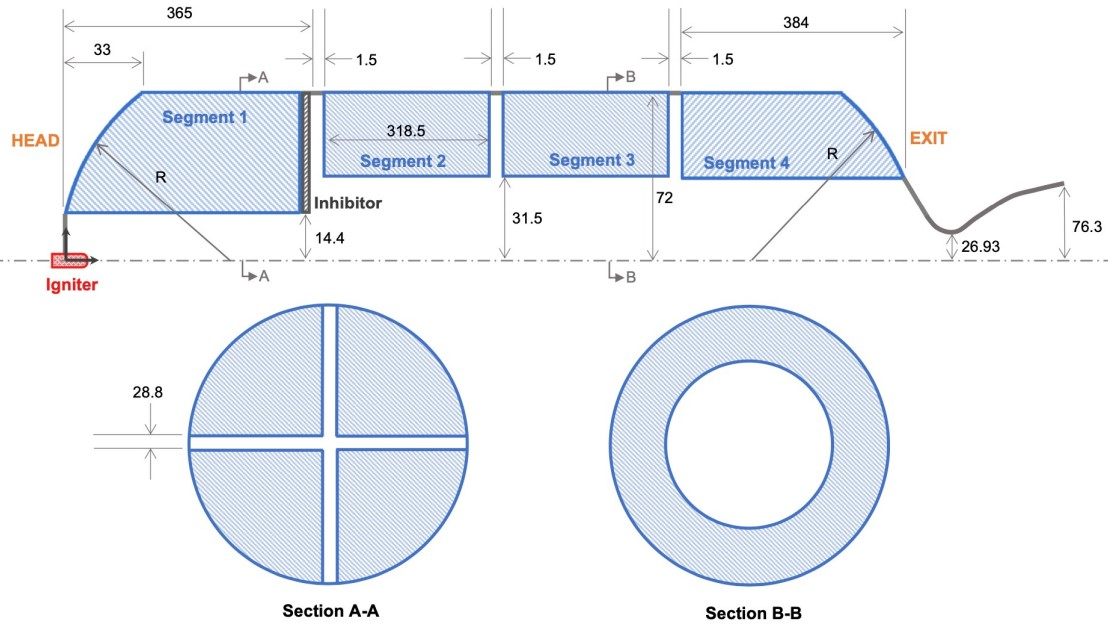
\includegraphics[width=0.85\textwidth]{images/prop-grain-section}
    \caption{Cross section of model shuttle solid rocket booster, with different grain geometries highlighted}
    \label{figure:srm-cross-section}
\end{figure}

After the convergence of the system of equations and termination, certain compressible flow losses can be seen from the results of the program as shown by \Cref{figure:model-chamber-pressure}. As the motor burned, the Mach number decreased, shown in \Cref{figure:mach-through-motor}, which led to less total pressure loss, and ultimately less entropy generation. The port area dictates the flow's Mach number which if high enough, leads to compressible effects and erosive burning. This is typically around Mach 0.3.

\begin{figure}
    \centering
    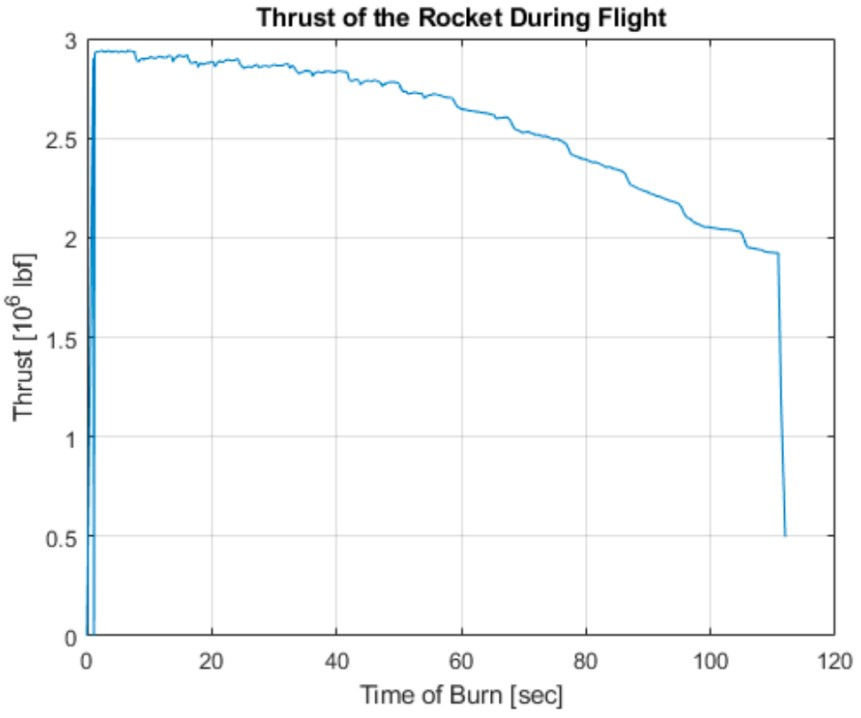
\includegraphics[width=0.48\textwidth]{images/combustion-thrust-v-time}
    \hfill
    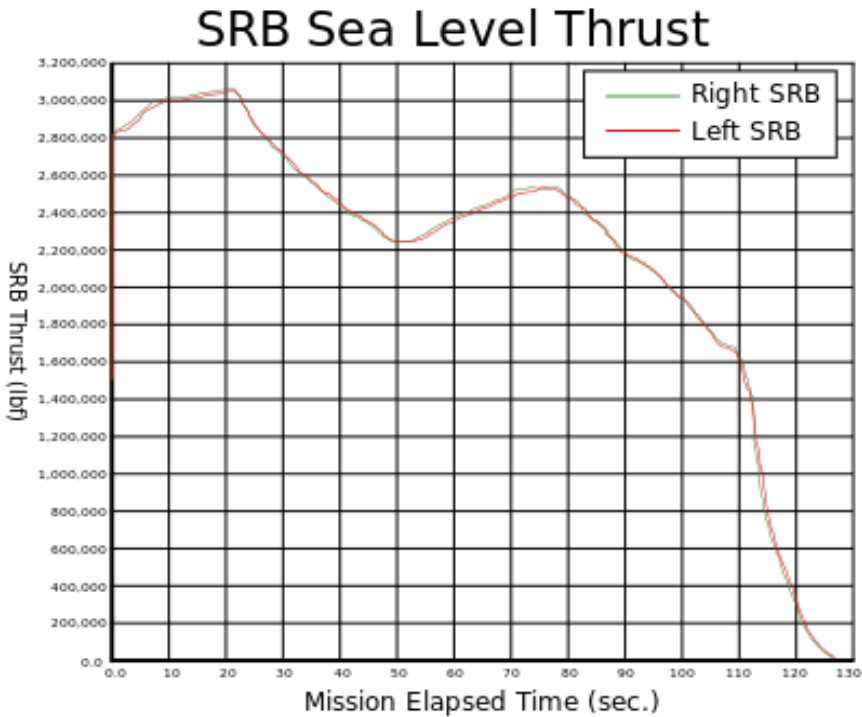
\includegraphics[width=0.48\textwidth]{images/srb-thrustcurve}
    \caption{Thrust curve produced by our model, compared to the true thrust curve of the Space Shuttle SRBs}
    \label{figure:thrustcurve-comparison}
\end{figure}

While the thrust profile of the model was similar when compared to the published data from the Space Shuttle, some key differences are noticeable. This is because the actual booster had an 11-pointed star grain geometry whereas the model uses a simple cross geometry. Additionally, erosive burning was not accounted for due to the relatively low Mach throughout the port. However, the magnitude of thrust for the max Q range between 20 - 75 seconds is highly comparable between the model and the actual results.

It was found that Mach number decreases in the slot elements due to stagnation pressure loss and the increase in cross sectional area while Mach Increases down the port due to heat and mass addition.

Rate of the mass flow rate accumulation changes as a function of time for each segment due to the surface area of the segment changing. It can be seen comparing the initial slope visually to the slope after a period of time that segment 1 burns regressively since its slope decreases with time and segments 2-4 burn progressively since their slope increases with time. As the segments burn axially in the slotted regions, the slotted region grows, and no mass is accumulated in that region.

\begin{figure}
    \centering
    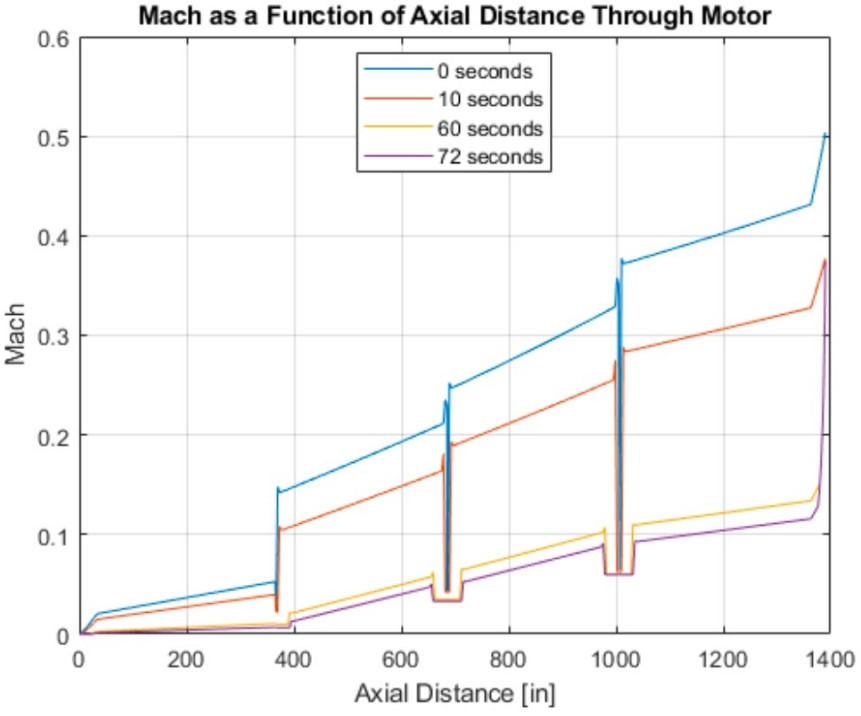
\includegraphics[width=0.65\textwidth]{images/mach-through-motor}
    \caption{Mach number through each element's port}
    \label{figure:mach-through-motor}
\end{figure}

\begin{figure}
    \centering
    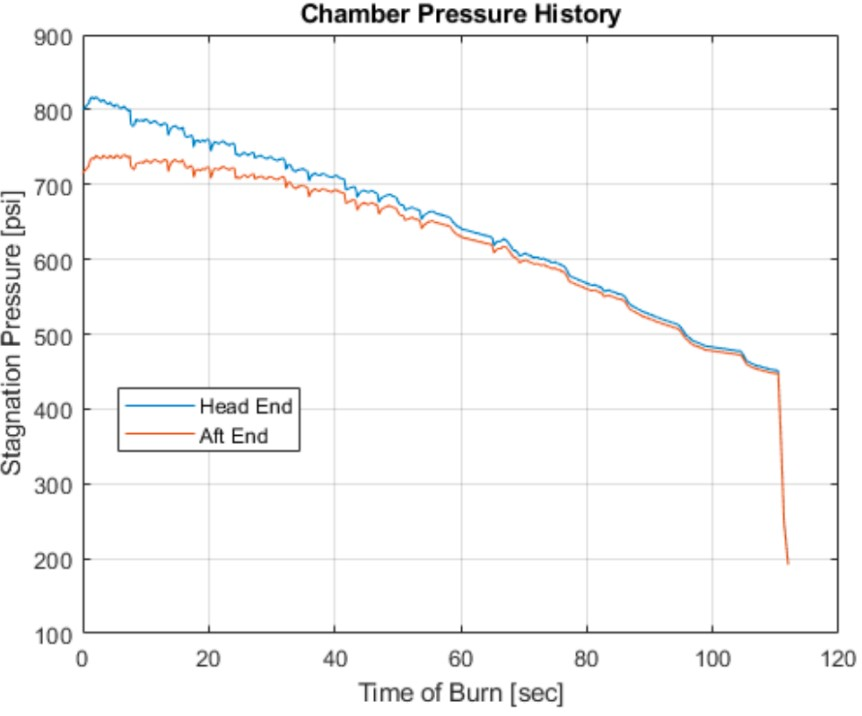
\includegraphics[width=0.65\textwidth]{images/combustion-chamber-pressure}
    \caption{Model chamber pressure}
    \label{figure:model-chamber-pressure}
\end{figure}

\begin{figure}
    \centering
    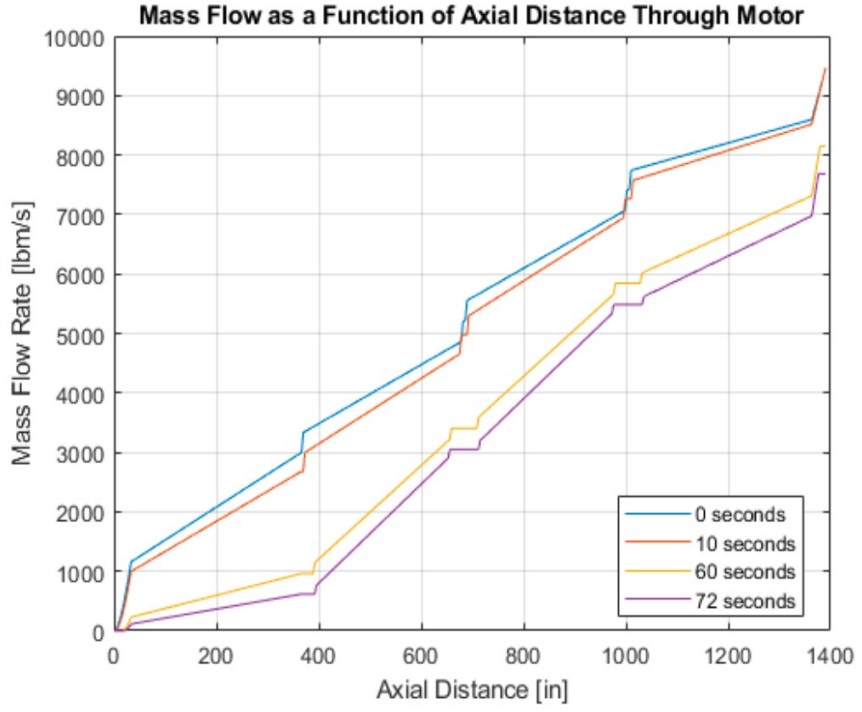
\includegraphics[width=0.65\textwidth]{images/massflow-through-motor}
    \caption{Model mass flow}
    \label{figure:massflow-through-motor}
\end{figure}

Ultimately by using the Space Shuttle as a case study, and comparing it to real data, we are able to build confidence in our ballistics code. In the future this program will be utilized to match grain geometries to chamber pressure profiles from selected point designs. There are a near infinite number of grain geometries to fit a pressure curve, but using intuition on manufacturability and prior art on geometries we will hopefully be able to deduce what the geometry could look like. Furthermore, this model will be used after Bates testing has been done with our chosen propellant in order to update burn rates, chamber pressure, and thrust as a function of time. With more accurate data, in the future this model could be improved by adding an erosive burn rate modifier by using Green’s model \(r = a P_c^n (1 + k M)\), where \(k\) is found experimentally.